\documentclass[tikz,border=2pt]{standalone}
\usepackage{fontspec}
\setmainfont{Times New Roman}
\usepackage{amsmath,amssymb}
\usetikzlibrary{arrows.meta}

\begin{document}
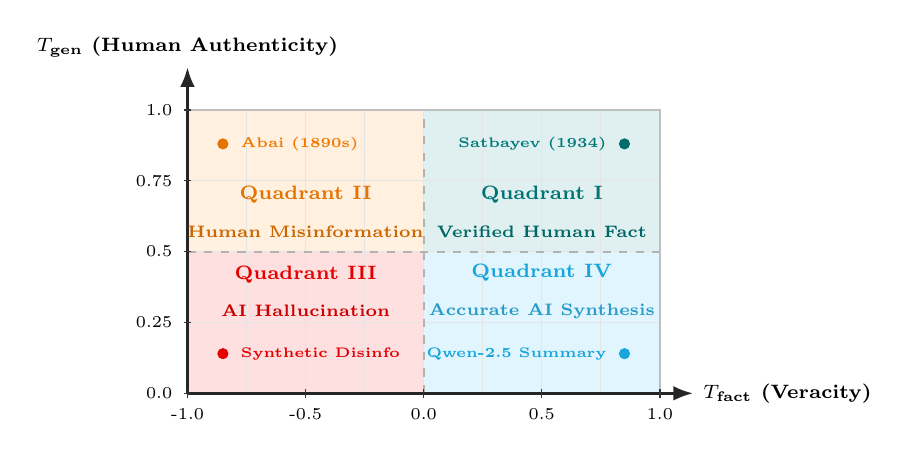
\begin{tikzpicture}[
    >=Latex,
    x=3.0cm,
    y=3.6cm
]

% 1. Quadrant Background Shading
% Q1: Upper-Right (Teal/Emerald)
\fill[teal!12] (0, 0.5) rectangle (1.0, 1.0);
% Q2: Upper-Left (Amber/Orange)
\fill[orange!12] (-1.0, 0.5) rectangle (0, 1.0);
% Q3: Lower-Left (Crimson/Red)
\fill[red!12] (-1.0, 0) rectangle (0, 0.5);
% Q4: Lower-Right (Cyan/Blue)
\fill[cyan!12] (0, 0) rectangle (1.0, 0.5);

% 2. Subtle Grid
\draw[gray!20, step=0.25, line width=0.3pt] (-1.0, 0) grid (1.0, 1.0);

% 3. Quadrant Division Lines (Dashed decision thresholds)
\draw[line width=0.7pt, draw=gray!60, dashed] (-1.0, 0.5) -- (1.0, 0.5);
\draw[line width=0.7pt, draw=gray!60, dashed] (0, 0) -- (0, 1.0);

% 4. Outer Boundary Frame
\draw[line width=0.6pt, draw=gray!50] (-1.0, 0) rectangle (1.0, 1.0);

% 5. Primary Axes with Arrows
% Veracity Axis along bottom
\draw[->, line width=0.9pt, draw=black!85] (-1.0, 0) -- (1.14, 0) 
    node[right, font=\fontsize{7pt}{8pt}\selectfont\bfseries] {$T_{\text{fact}}$ (Veracity)};
% Authenticity Axis along left
\draw[->, line width=0.9pt, draw=black!85] (-1.0, 0) -- (-1.0, 1.15) 
    node[above, font=\fontsize{7pt}{8pt}\selectfont\bfseries] {$T_{\text{gen}}$ (Human Authenticity)};

% 6. Ticks and Labels
% X-axis ticks (along y=0)
\foreach \x in {-1.0, -0.5, 0.0, 0.5, 1.0} {
    \draw[line width=0.5pt, draw=black!80] (\x, 0.015) -- (\x, -0.015);
    \node[below=2pt, font=\fontsize{6pt}{7pt}\selectfont] at (\x, 0) {\x};
}
% Y-axis ticks (along x=-1.0)
\foreach \y in {0.0, 0.25, 0.5, 0.75, 1.0} {
    \draw[line width=0.5pt, draw=black!80] (-0.985, \y) -- (-1.015, \y);
    \node[left=2pt, font=\fontsize{6pt}{7pt}\selectfont] at (-1.0, \y) {\y};
}

% 7. Quadrant Titles (2-line bold and legible, centered in each quadrant)
% Q1: Upper-Right (centered at (0.50, 0.64))
\node[align=center] at (0.50, 0.64) {
    \textbf{\fontsize{7pt}{8pt}\selectfont\color{teal!90!black}Quadrant I}\\[1.5pt]
    \textbf{\fontsize{6.2pt}{7.2pt}\selectfont\color{teal!80!black}Verified Human Fact}
};

% Q2: Upper-Left (centered at (-0.50, 0.64))
\node[align=center] at (-0.50, 0.64) {
    \textbf{\fontsize{7pt}{8pt}\selectfont\color{orange!90!black}Quadrant II}\\[1.5pt]
    \textbf{\fontsize{6.2pt}{7.2pt}\selectfont\color{orange!80!black}Human Misinformation}
};

% Q3: Lower-Left (centered at (-0.50, 0.36))
\node[align=center] at (-0.50, 0.36) {
    \textbf{\fontsize{7pt}{8pt}\selectfont\color{red!90!black}Quadrant III}\\[1.5pt]
    \textbf{\fontsize{6.2pt}{7.2pt}\selectfont\color{red!80!black}AI Hallucination}
};

% Q4: Lower-Right (centered at (0.50, 0.36))
\node[align=center] at (0.50, 0.36) {
    \textbf{\fontsize{7pt}{8pt}\selectfont\color{cyan!90!black}Quadrant IV}\\[1.5pt]
    \textbf{\fontsize{6.2pt}{7.2pt}\selectfont\color{cyan!80!black}Accurate AI Synthesis}
};

% 8. Forensic Benchmark Sample Markers with Lateral Labels
% Sample 1: Q1 (Satbayev 1934) at (0.85, 0.88)
\filldraw[teal!85!black] (0.85, 0.88) circle (1.8pt);
\node[left=3pt, font=\fontsize{5.2pt}{6pt}\selectfont\bfseries, text=teal!95!black] at (0.85, 0.88) {Satbayev (1934)};

% Sample 2: Q2 (Abai 1890s) at (-0.85, 0.88)
\filldraw[orange!90!black] (-0.85, 0.88) circle (1.8pt);
\node[right=3pt, font=\fontsize{5.2pt}{6pt}\selectfont\bfseries, text=orange!95!black] at (-0.85, 0.88) {Abai (1890s)};

% Sample 3: Q3 (Synthetic Disinfo) at (-0.85, 0.14)
\filldraw[red!90!black] (-0.85, 0.14) circle (1.8pt);
\node[right=3pt, font=\fontsize{5.2pt}{6pt}\selectfont\bfseries, text=red!90!black] at (-0.85, 0.14) {Synthetic Disinfo};

% Sample 4: Q4 (Qwen Summary) at (0.85, 0.14)
\filldraw[cyan!90!black] (0.85, 0.14) circle (1.8pt);
\node[left=3pt, font=\fontsize{5.2pt}{6pt}\selectfont\bfseries, text=cyan!90!black] at (0.85, 0.14) {Qwen-2.5 Summary};

\end{tikzpicture}
\end{document}
